
\documentclass[fleqn,addpoints]{exam}

\usepackage{units} 
\usepackage{graphicx}
\usepackage[fleqn]{amsmath}
\usepackage{cancel}
\usepackage{float}
\usepackage{mdwlist}
\usepackage{booktabs}
\usepackage{cancel}
\usepackage{polynom}
\usepackage{caption}
\usepackage{fullpage}
\usepackage{xfrac}
\usepackage{enumerate}

\everymath{\displaystyle}

\printanswers

\ifprintanswers
  \usepackage{2in1, lscape}
\fi

\title{Math 141 Chapter Two Exam}
\date{March 6, 2013}
\author{}

\begin{document}

\maketitle  

\ifprintanswers
  \else
  \vspace{0.2in}
  \makebox[\textwidth]{Name:\enspace\hrulefill}
  \vspace{0.2in}

  \begin{center}
  \gradetable[h][pages]
  \bonusgradetable[h][pages]
  \end{center}
\fi

\vspace{1 cm} 

\begin{questions}
  % \uplevel{ \section{Graphing} }

  \ifprintanswers
  \else
    \pagebreak
  \fi

  \question[5]
    Find the domain of each function:
    \begin{parts}

      \part[3] $f(x) = \sqrt{x - 3}$
      \begin{solution}[4 cm]
        \begin{align*}
          x - 3 &\geq 0 \\
          x     &\geq 3 \\
        \end{align*}

        $[3, \infty)$

      \end{solution}

      \part[7] $f(x) = \sqrt{x^2 - 2x - 8}$
      \begin{solution}[8 cm]
        \begin{align*}
          x^2 - 2x - 8   &\geq 0 \\
          (x - 4)(x + 2) &\geq 0 \\
        \end{align*}

        The domain is: $(-\infty, -2] \cup [4, \infty)$

      \end{solution}

      \part[7] $f(x) = \frac{x^2 + 2x - 3}{\sqrt{4 - x^2}}$
      \begin{solution}
        Any number will work for the numerator, so the only thing that matters is the denominator.
        \begin{align*}
          4 - x^2 &> 0 \\
          x^2     &< 4 \\
          |x|     &< 2 \\
        \end{align*}

        The domain is: $(-2, 2)$

      \end{solution}

    \end{parts}

  \ifprintanswers
  \else
    \pagebreak
  \fi

  \question
    $f(x) = \frac{x^2}{|2x|}$

    \begin{parts}
      \part[2] What is the domain of $f$?
        \begin{solution}[1 cm]
          $x \neq 0$
        \end{solution}

      \part[5]
        Graph $f$.

          \begin{figure}[H]
            \centering
            \ifprintanswers
              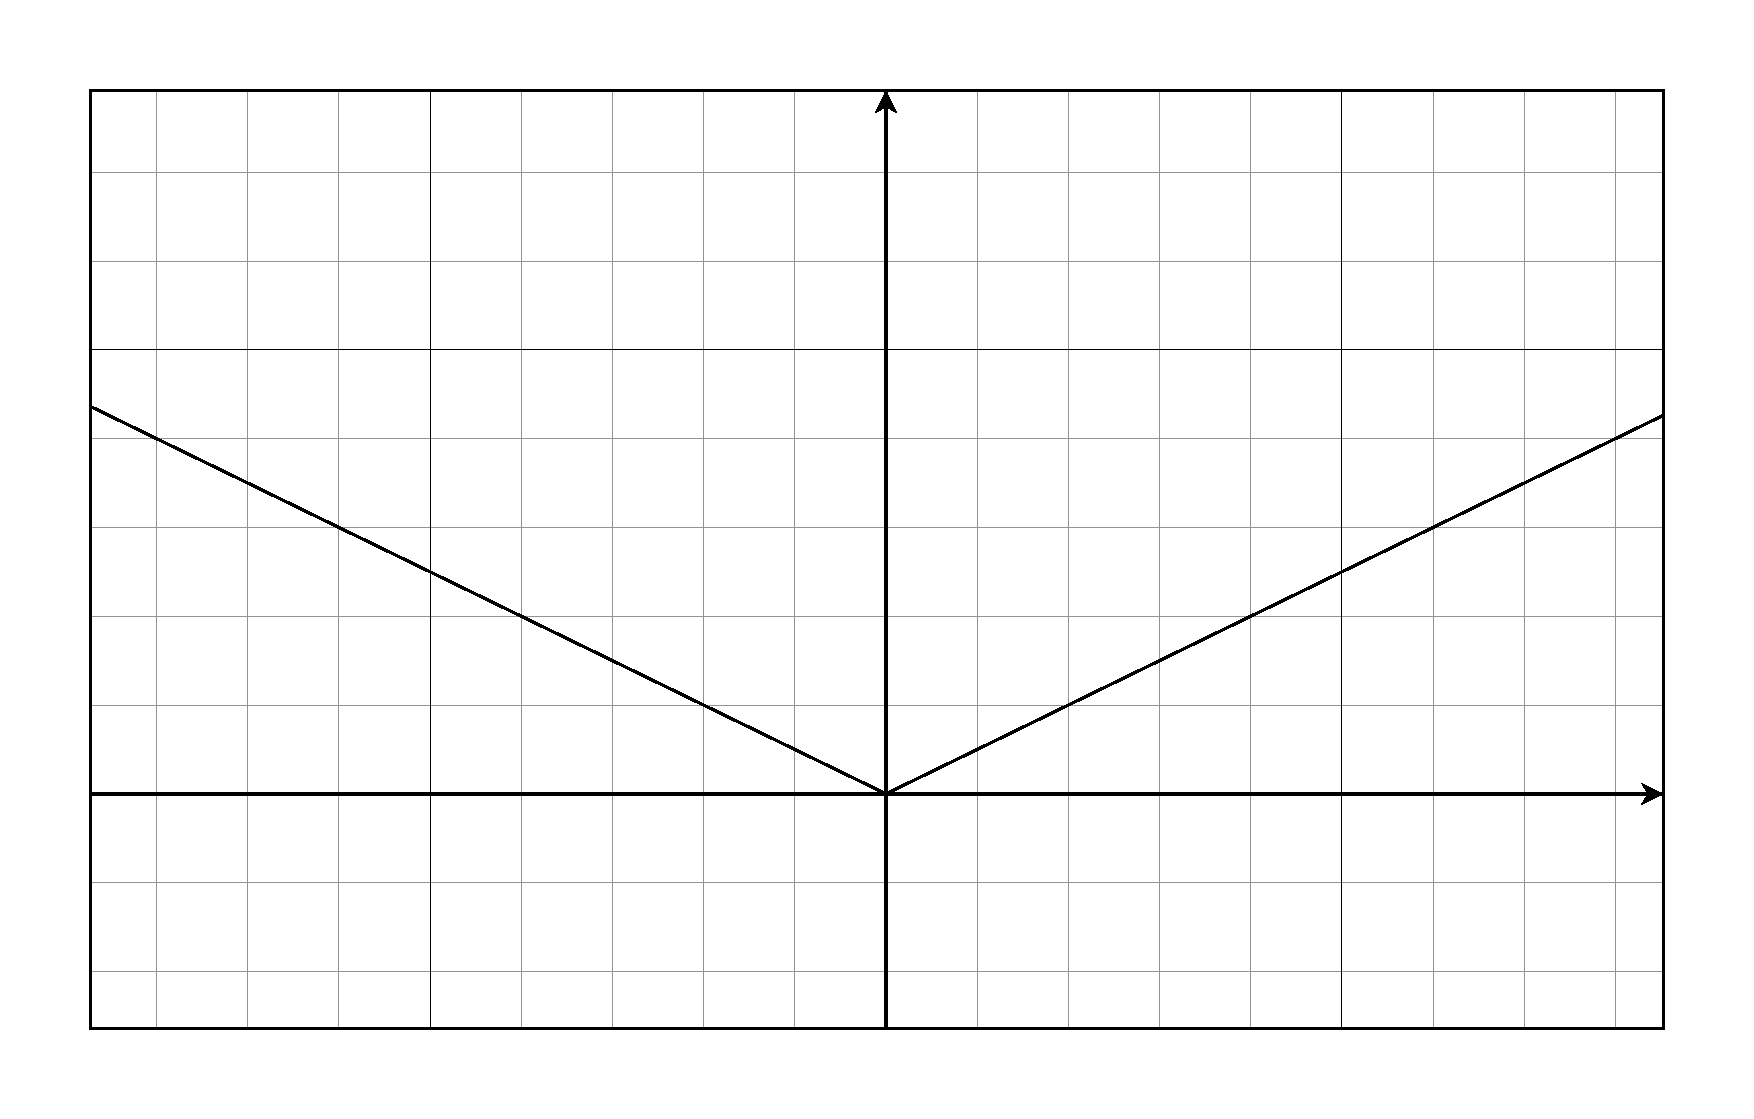
\includegraphics[scale=.4]{problem_2_solution.eps}
            \else
              \includegraphics[scale=.6]{problem_2_blank.eps}
            \fi
            \caption*{Problem 2}
          \end{figure}

    \end{parts}

  \ifprintanswers
  \else
    \pagebreak
  \fi

  \question
    \[
      f(x) = 
        \begin{cases}
          x       & \text{if } x \geq 0 \\
          4 - x^2 & \text{if } x < 0 \\
        \end{cases}
    \]

    \begin{parts}
      \part[2] What is the domain of $f$?
        \begin{solution}[1 cm]
          $(-\infty, \infty)$
        \end{solution}

      \part[5]
        Graph $f$.

        \begin{figure}[H]
          \centering
          \ifprintanswers
            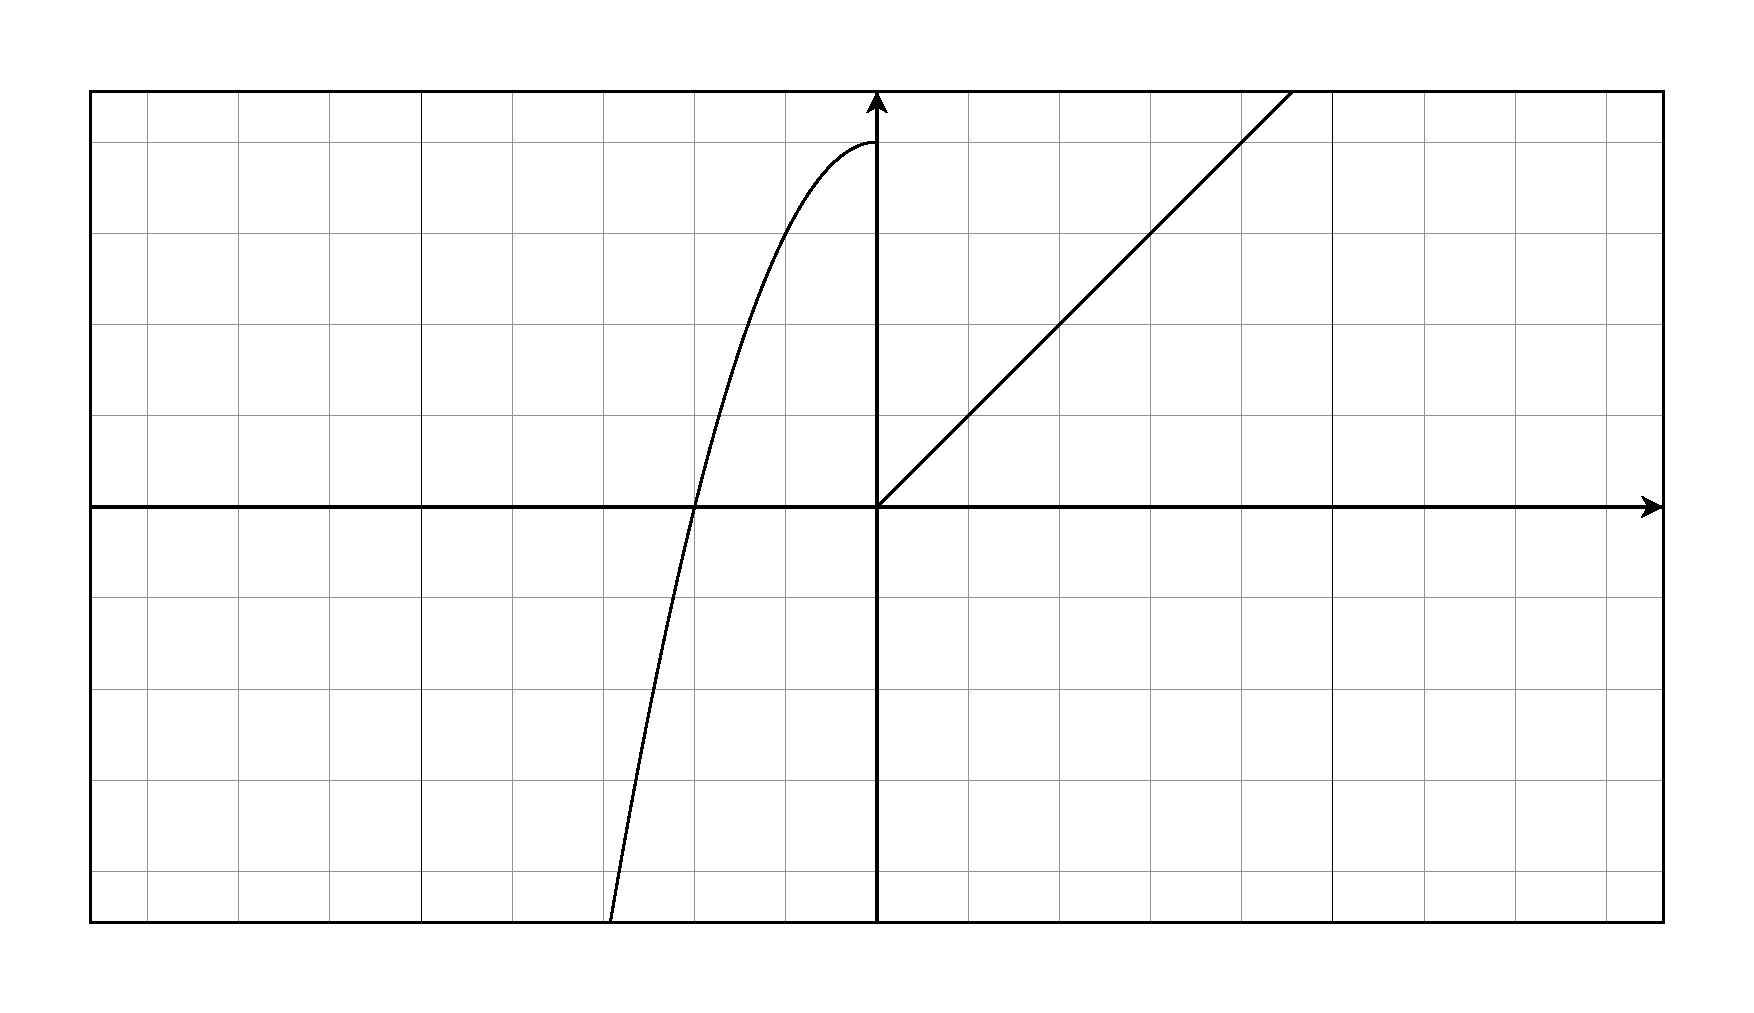
\includegraphics[scale=.4]{problem_3_solution.eps}
          \else
            \includegraphics[scale=.6]{problem_3_blank.eps}
          \fi
          \caption*{Problem 3}
        \end{figure}

    \end{parts}

  \ifprintanswers
  \else
    \pagebreak
  \fi

  \question[5]
    Determine the average rate of change for $f(x) = x^3 + 1$ between $x = -2$ and $x = 2$.
    \begin{solution}[5 cm]
      \begin{align*}
        f_{avg} &= \frac{f(2) - f(-2)}{2 - (-2)} \\
                &= \frac{9 - (-7)}{4} \\
                &= 4 \\
      \end{align*}
    \end{solution}

  \question Show that the function is even, odd, or neither.
    \begin{parts}

      \part[5] $f(x) = \frac{1}{x} - x^3$
        \begin{solution}[6 cm]
          \begin{align*}
            f(-x) &= \frac{1}{-x} - (-x)^3 \\
                  &= -\frac{1}{x} + x^3 \\
                  &= -\left(\frac{1}{x} - x^3 \right) \\
                  &= - f(-x) \\
          \end{align*}

          Since $f(-x) = -f(x)$, this function is odd.
        \end{solution}
      
  \ifprintanswers
    \pagebreak
  \fi
      \part[5] $f(x) = (x - 1)^2$
        \begin{solution}[5 cm]
          \begin{align*}
            f(x) &= (x - 1)^2 \\
                 &= x^2 - 2x + 1 \\
            \\
            f(-x) &= (-x)^2 - 2(-x) + 1 \\
                  &= x^2 + 2x + 1 \\
          \end{align*}

          Since $f(-x) \neq -f(x)$ and $f(-x) \neq f(x)$, this function is neither odd nor even.

          Another way to see this one is that the function is a parabola shifted left by 1, so it won't be symmetric
          around either the y-axis or the origin.

        \end{solution}

    \end{parts}

  \ifprintanswers
  \else
    \pagebreak
  \fi

  \question
    Suppose the graph of $f$ is given.  Describe how the graph of each function can be obtained from the graph of $f$
    ({\em shift left 7 and down 12}, etc.).
    
    \begin{parts}
      \part[2] $g(x) = f(x) + 2$
        \begin{solution}[4 cm]
          shift up 2
        \end{solution}

      \part[2] $g(x) = f(x - 2)$
        \begin{solution}[4 cm]
          shift right 2
        \end{solution}

      \part[2] $g(x) = 3f(-x)$
        \begin{solution}[4 cm]
          reflect around the y-axis and scale vertically by 3
        \end{solution}

%       \part[2] $g(x) = -f(2x)$
%         \begin{solution}[2 cm]
%         \end{solution}
% 
      \part[2] $g(x) = f(x + 2) - 3$
        \begin{solution}[4 cm]
          shift left 2 and down 3
        \end{solution}

    \end{parts}

  \ifprintanswers
  \else
    \pagebreak
  \fi

  \question[4]
    Match each equation with a graph.

    \ifprintanswers
      \begin{solution}
        \begin{tabular}{ll}
          \toprule
          equation                         & graph \\
          \midrule
          $y = (x + 1)^2$                  & B     \\
          \midrule
          $y = -(x - 1)^2 + 1$             & C     \\
          \midrule
          $y = 4(x + 5)^2 - 2$             & A     \\
          \midrule
          $y = - \frac{1}{4}(x - 4)^2 + 2$ & D     \\
          \bottomrule
        \end{tabular}
      \end{solution}
    \else
      \begin{tabular}{ll}
        \toprule
        equation                         & graph \\
        \midrule
        $y = (x + 1)^2$                  & \\
        \midrule
        $y = -(x - 1)^2 + 1$             & \\
        \midrule
        $y = 4(x + 5)^2 - 2$             & \\
        \midrule
        $y = - \frac{1}{4}(x - 4)^2 + 2$ & \\
        \bottomrule
      \end{tabular}
    \fi


  \begin{figure}[H]
    \centering
    \ifprintanswers
      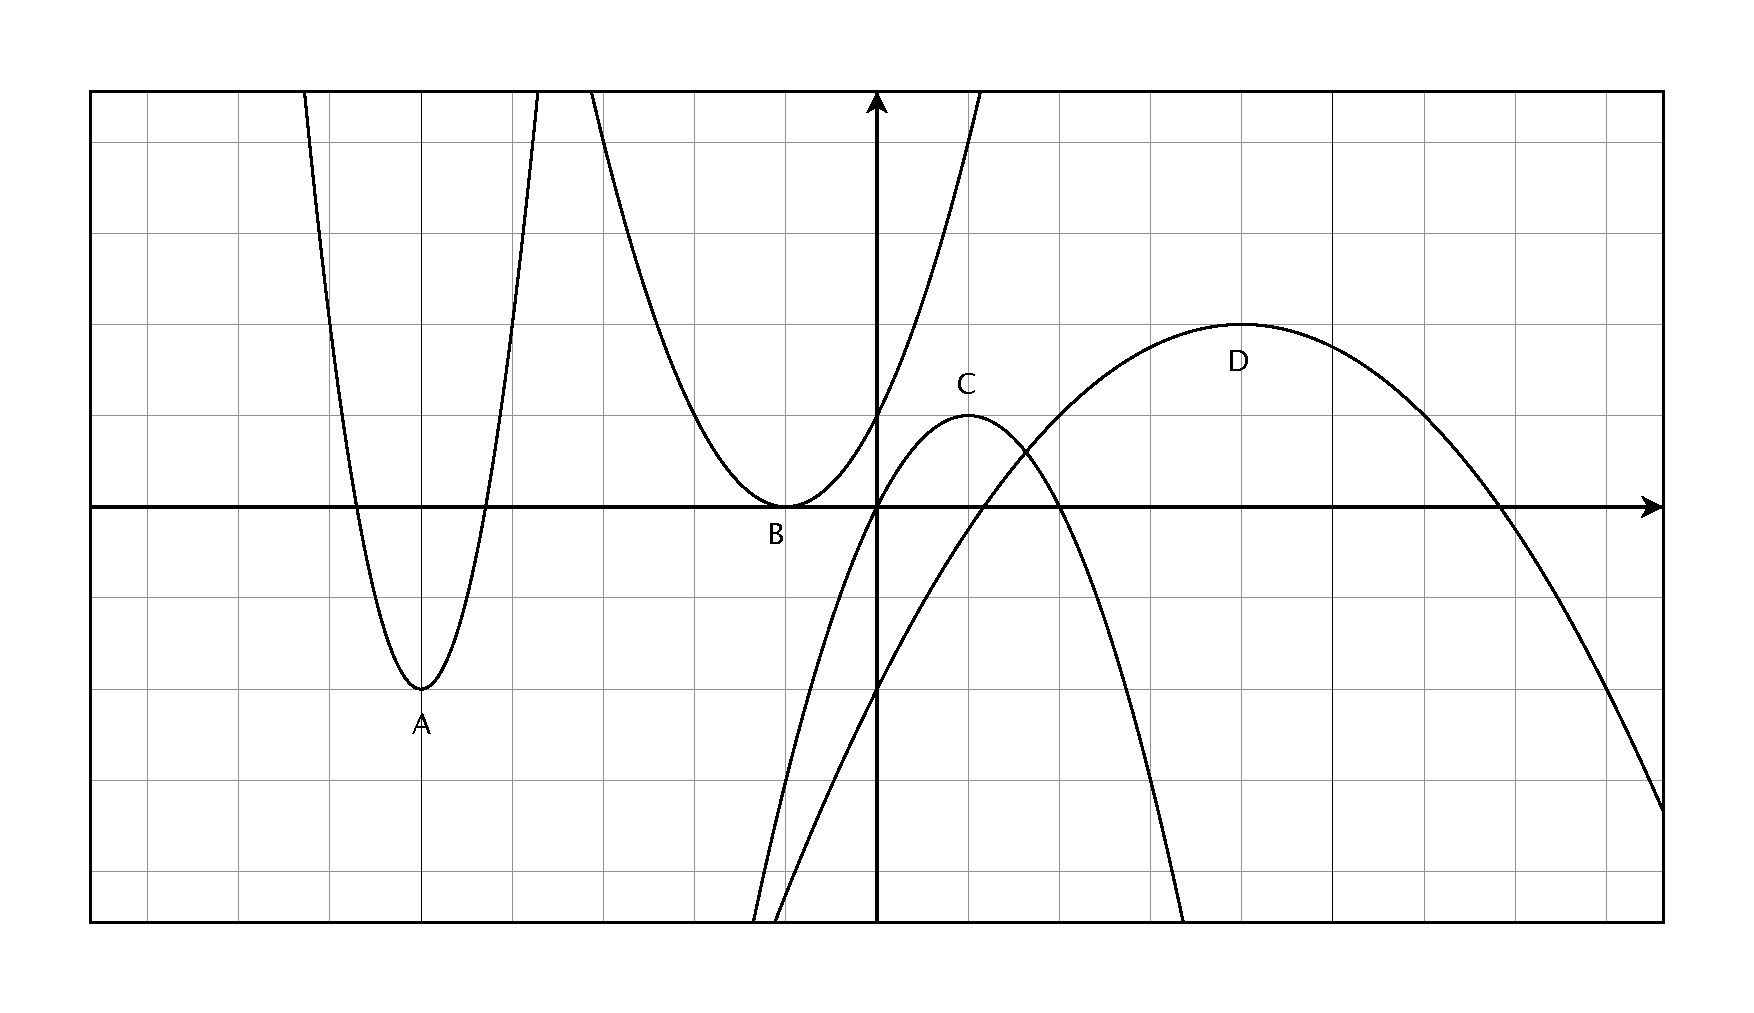
\includegraphics[scale=.4]{problem_7.eps}
    \else
      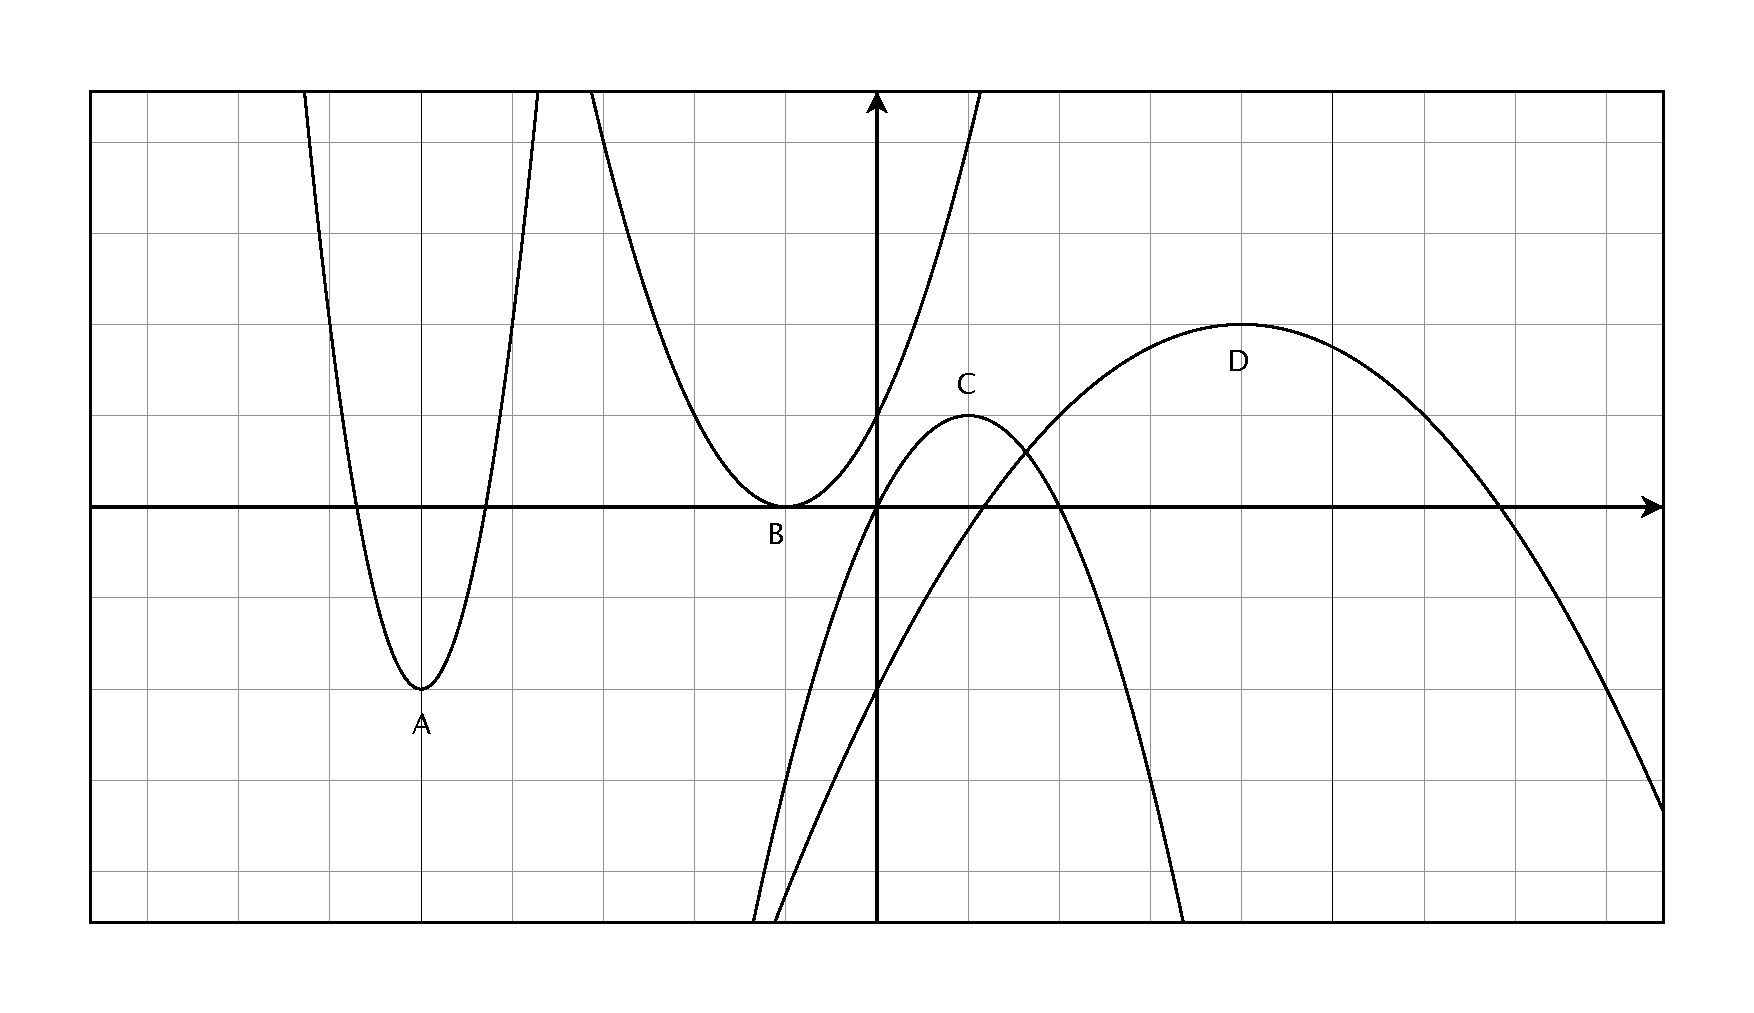
\includegraphics[scale=.6]{problem_7.eps}
    \fi
    \caption*{Problem 7}
  \end{figure}

  \ifprintanswers
  \else
    \pagebreak
  \fi

  \ifprintanswers
    \pagebreak
  \fi

  \question[5] Graph $f(x) = (x + 1)^2 - 4$
    \vspace{1 cm}
    \begin{figure}[H]
      \centering
      \ifprintanswers
        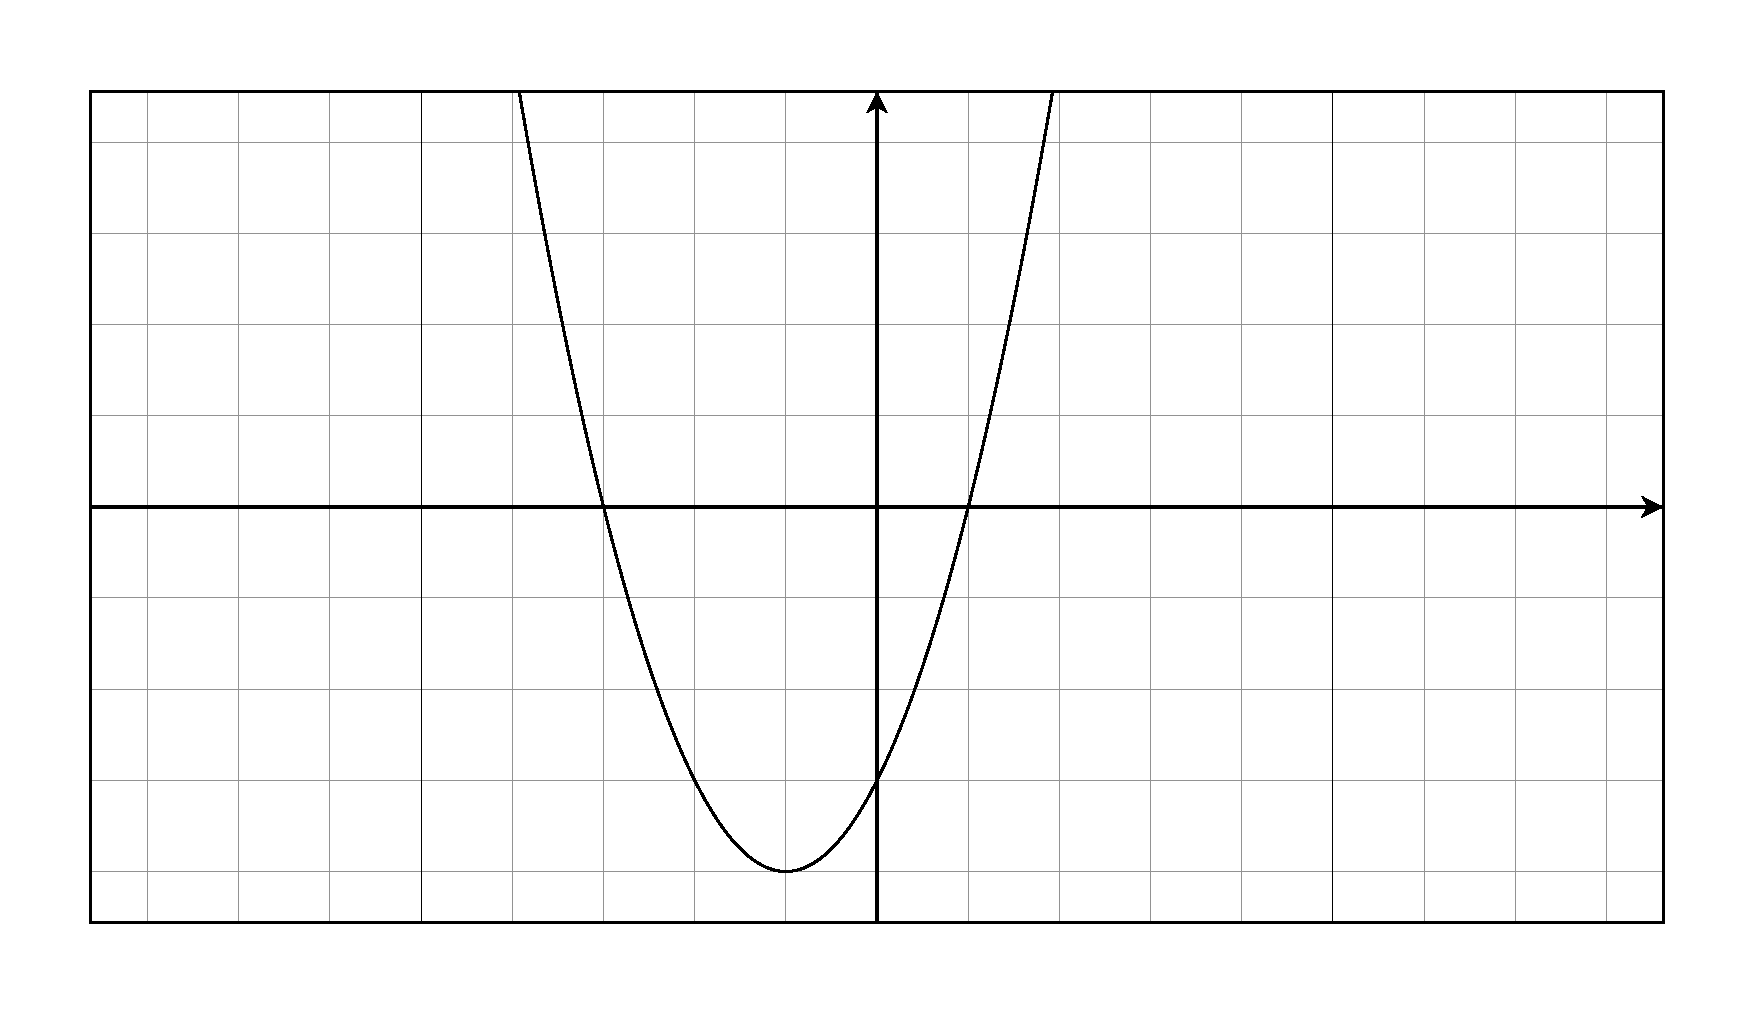
\includegraphics[scale=.4]{problem_8_solution.eps}
      \else
        \includegraphics[scale=.6]{problem_8_blank.eps}
      \fi
      \caption*{Problem 8}
    \end{figure}

  \ifprintanswers
  \else
    \pagebreak
  \fi

  \question Put $f$ in standard form.
    \begin{parts}
      \part[7]
        \[
          f(x) = x^2 -6x + 14
        \]

        \begin{solution}[8 cm]
          \[
            (x - 3)^2 + 5
          \]
        \end{solution}

  \ifprintanswers
    \pagebreak
  \fi

      \part[7]
        \[
          f(x) = -2x^2 + 4x + 1
        \]

        \begin{solution}
          \[
            -2(x - 1)^2 + 3
          \]
        \end{solution}
    \end{parts}

  \ifprintanswers
  \else
    \pagebreak
  \fi

  \question[7] Find the maximum value of $f(x) = -x^2 + 4x - 3$.
    \begin{solution}[6 cm]
      \begin{align*}
        x_{max} &= \frac{-4}{2 \cdot (-1)} = 2 \\
        f(2)    &= 1 \\
      \end{align*}
    \end{solution}

  \ifprintanswers
    \pagebreak
  \fi

  \question[10]
    % Schwam's outline, pg. 100

    Hagrid has retired from his gamekeeper job at Hogwarts and taken up farming.  He plans to raise hippogriffs and
    Blast-Ended Skrewts.  Of course, he needs to keep the skrewts and hippogriffs separated so they don't eat each
    other.
    
    He's planning to build a rectangular field to hold the animals.  Since he wants them to have a regular water
    supply, he's going to have one side of the field on the river which runs through his farm.  This means that he only
    needs to fence the remaining three sides of the rectangle and include a divider.  What are the dimensions of the
    largest area field he can construct with 90 feet of fence?

    \begin{solution}[9 cm]
      If the sides perpendicular to the river are $x$ and the side parallel to the river is $y$:
      \begin{align*}
        90 &= 3x + y \\
        y  &= 90 - 3x \\
      \end{align*}

      The area is:
      \[
        A = xy
      \]

      Plug $y$ into the area equation to get a function of $x$:
      \begin{align*}
        A &= x(90 - 3x) \\
        90 - 3x^2 + 90x \\
      \end{align*}
      The $x$ value which produces the maximum area is:
      \[
        x_{max} = \frac{-90}{2 \cdot (-3)} = 15
      \]

      The $y$ value is the amount of fence left over:
      \[
        y = 90 - 3 \cdot 15 = 45
      \]

      A field with $x = 15$ and a $y = 45$ will have the largest possible area.

    \end{solution}

  \ifprintanswers
  \else
    \pagebreak
  \fi

  \question
    \begin{align*}
      f(x) &= \frac{1}{x} \\
      g(x) &= \sqrt{x + 2} \\
    \end{align*}

    Find each function and its domain:

    \begin{parts}
      \part[3] $(f + g)(x)$
        \begin{solution}[3 cm]
          $(f + g)(x) = \frac{1}{x} + \sqrt{x + 2}$;
          
          Domain: $[-2, 0) \cup (0, \infty)$
        \end{solution}
      
      \part[3] $(f / g)(x)$
        \begin{solution}[3 cm]
          $(f / g)(x) = \frac{1}{x \sqrt{x + 2}}$

          Domain: $(-2, 0) \cup (0, \infty)$
        \end{solution}

      \part[3] $(f \circ g)(x)$
        \begin{solution}[3 cm]
          $(f \circ g)(x) = \frac{1}{\sqrt{x + 2}}$

          Domain: $(-2, \infty)$
        \end{solution}

      \part[3] $(f \circ f)(x)$
        \begin{solution}[3 cm]
          $(f \circ f)(x) = \frac{1}{1/x} = x$

          Domain: $x \neq 0$
        \end{solution}

    \end{parts}

  \pagebreak

  \question[5]
    How could you restrict the domain of $f(x) = (x - 2)^2 + 1$ to make $f$ one-to-one?
    \begin{solution}[4 cm]
      This is the graph of a parabola shifted right by 2 and up by 1.  If you restrict the domain to $x \geq 2$, you
      only end up with the right half of the parabola so the function becomes one-to-one.
    \end{solution}

  \question
    Find $f^{-1}$ and its domain:
    \begin{parts}
      \part[7] $\frac{3x + 2}{2x - 5}$
        \begin{solution}[8 cm]
          \begin{align*}
            y         &= \frac{3x + 2}{2x - 5} \\
            2xy - 5y  &= 3x + 2 \\
            2xy - 3x  &= 5y + 2 \\
            x(2y - 3) &= 5y + 2 \\
            x         &= \frac{5y + 2}{2y - 3} \\
            \\
            f^{-1}(x) &= \frac{5x + 2}{2x - 3} \\
          \end{align*}

          $x \neq \frac{3}{2}$
        \end{solution}

      \part[7] $x^2 + 2x + 1$
        \begin{solution}
          I forgot to restrict the domain of this to $x \geq -1$.  Without restricting the domain, there isn't an
          inverse.  Assuming the domain is restricted, here's the solution:
          \begin{align*}
            y         &= x^2 + 2x + 1 \\
                      &= (x + 1)^2 \\
            \sqrt{y}  &= x + 1 \\
            x         &= \sqrt{y} - 1 \\
            \\
            f^{-1}(x) &= \sqrt{x} - 1 \\
          \end{align*}

          $x \geq 0$

        \end{solution}
  \end{parts}

  \pagebreak

  \uplevel{\section{Extra Credit}}

  \bonusquestion
    Hagrid's hippogriff farm is thriving and he's decided to start renting the hippogriffs out for rides.  His business
    does well and in the first year he serves 5,000 customers by charging \$30 per ride.

    Hagrid wants to make sure he's charging the optimal rate for rides, so he hires Hermione as a consultant.  She
    determines that each dollar added to the rental rate results in a loss of 500 customers per year and each dollar
    subtracted from the rental rate results in 500 more customers per year.

%     A cable TV company serves 5,000 customers and charges \$30 per month.  They did a marketing survey, and discovered
%     that adding a dollar to the monthly rate results in a loss of 500 customers and lowering the monthly rate by a
%     dollar results in a gain of 500 customers.

    \begin{parts}
      \bonuspart[10] Find the revenue function $R(x)$ which determines the revenue when the rental rate is
        $\unit[x]{dollars}$.

        \begin{solution}[8 cm]
          The number of customers when the rate is $x$ dollars is: 
          \begin{align*}
            C(x) &= 5,000 + 500(30 - x) \\
                 &= 20,000 - 500x \\
          \end{align*}

          Each customer pays $x$ per rental, so the revenue function is
          \begin{align*}
            R(x) &= (20,000 - 500x)x \\
                 &= -500x^2 + 20,000 x \\
          \end{align*}
        \end{solution}

  \ifprintanswers
    \pagebreak
  \fi

      \bonuspart[5] What rental rate results in the maximum revenue?
        \begin{solution}[4 cm]
          The maximum revenue occurs when:
          \[
            x = \frac{-20,000}{2 \cdot (-500)} = \$20
          \]

          With this rental rate, Hagrid's revenue is:
          \[
            R(20) = \$200,000 \\
          \]

          Of course, he still has to feed the hippogriffs and pay Hermione, so it isn't all profit.

        \end{solution}

    \end{parts}

\end{questions}

\end{document}
